\documentclass{xStandalone}

\begin{document}
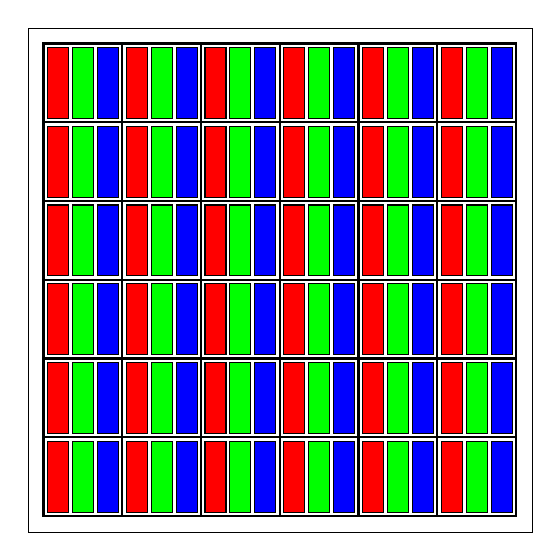
\begin{tikzpicture}

\def\sep{0.05}
\def\wid{\fpeval{(1-4*\sep)/3}}
\def\hei{\fpeval{(1-2*\sep)}}
    
\foreach \x in {0,1,...,5}
{
    \foreach \y in {0,1,...,5}
    {
        \draw[thick] (\x,\y) rectangle ++ (1,1);
        \draw[thin,fill=red] (\x,\y) ++(\fpeval{1*\sep+0*\wid},\sep) rectangle ++ (\wid,\hei);
        \draw[thin,fill=green] (\x,\y) ++(\fpeval{2*\sep+1*\wid},\sep) rectangle ++ (\wid,\hei);
        \draw[thin,fill=blue] (\x,\y) ++(\fpeval{3*\sep+2*\wid},\sep) rectangle ++ (\wid,\hei);
    }
}

\draw[ultra thin] (-0.2,-0.2) rectangle (6.2,6.2);

\end{tikzpicture}
\end{document}